\documentclass{beamer}
\usepackage[T1]{fontenc}
\usepackage[utf8]{inputenc}
\usepackage{lmodern} 
\usepackage[portuguese]{babel}
\usepackage{graphicx}			%para imagens
\usepackage{epstopdf} 			%resolve problemas eps-pdf
\usepackage{fancyhdr}			% para o cabeçalho bonito
\usepackage{caption}				%para legendas
\usepackage{placeins} 			%controlar o lugar dos floats
\usepackage{hyperref}
\usepackage{listings}
\usepackage{color}
\usepackage{xcolor}
\usepackage{tikz}

\definecolor{dkgreen}{rgb}{0,0.6,0}
\definecolor{gray}{rgb}{0.5,0.5,0.5}
\definecolor{mauve}{rgb}{0.58,0,0.82}

\lstset{frame=tb,
  language=Java,
  aboveskip=3mm,
  belowskip=3mm,
  showstringspaces=false,
  columns=flexible,
  basicstyle={\tiny\ttfamily},
  numbers=none,
  numberstyle=\tiny\color{gray},
  keywordstyle=\color{blue},
  commentstyle=\color{dkgreen},
  stringstyle=\color{mauve},
  breaklines=true,
  breakatwhitespace=true
  tabsize=3
}
\lstset{language=Java}

\defbeamertemplate*{title page}{customized}[1][]
{
  \usebeamerfont{title}\inserttitle\par
  \usebeamerfont{subtitle}\usebeamercolor[fg]{subtitle}\insertsubtitle\par
  \bigskip
 %% \usebeamerfont{author}\insertauthor\par
  \usebeamerfont{institute}\insertinstitute\par
  \usebeamerfont{date}\insertdate\par
  \usebeamercolor[fg]{titlegraphic}\inserttitlegraphic
}

%DEFINE TEMA BEAMER A SER UTILIZADO
\usetheme{Warsaw}
\setbeamertemplate{navigation symbols}{}%remove navigation symbols
%DEFINIÇÃO DE TÍTULO, AUTORES .....
\title[Introdução a Computação Sônica]{ ICS - Trabalho III \\ Efeito Risset Contínuo}
%\title[pequeno título que vai no bottom da página]{título grande}%
\author{Juarez Aires Sampaio Filho 11/0032829}
\institute{Universidade de Brasília}
\date{\today}

\begin{document}


\begin{frame}
        \titlepage
\end{frame}

\AtBeginSection[]
{
}
\section{Requisitos}
\begin{frame}{Requisitos}
	\begin{block}{}
	Utilizar as classes do pacote \textbf{sintese} para implementar o \emph{Paradoxo de Altura} e desenvolver uma interface gráfica conveniente e útil para a aplicação.
	\end{block}
\end{frame}

\section{Introdução Teórica}
\begin{frame}{Introdução Teórica 1/5}
\begin{itemize}
\item Implementou-se a versão contínua do efeito conhecida como \emph{Escala Risset Contínua}.
\item O efeito constitui-se de uma soma de senoides na forma:
\begin{equation}
	f(t) = \sum_{i} A_i(t) sin(2 \pi f_i(t))
\end{equation}
\item A relação A(f) deve implementar uma gaussiana em função do logaritmo da frequência
conforme a figura a seguir.
\end{itemize}
\end{frame}

\begin{frame}
 \frametitle{Introdução Teórica 2/5}
 \begin{figure}
  \includegraphics[scale=0.3]{./images/AxF.png}
  \caption{Relação Axf}
   \end{figure}
\end{frame}


\begin{frame}{Introdução Teórica 3/5}
\begin{itemize}
\item Escolhemos a função $f_i(t)$ de tal forma que ela caia a metade no instante $T_0$.
\item Escolhendo $f_{i_0} = f_0 2^i$, temos que $f_i(T_0) = f_{i-1}(0)$
\item Finalmente:
	\begin{equation}
		f_i(t) = f_{i_0}\cdot 2^{-\frac{t}{T_0}}
	\end{equation}
\end{itemize}
\end{frame}

\begin{frame}{Introdução Teórica 4/5}
\begin{itemize}
\item a Gaussiana logaritma é dada por:
	\begin{equation}
		A_i(t) = exp(-\frac{(\log f_i(t) - \log f_c)^2}{(2\sigma^2)})
	\end{equation}
\item substituindo:
	\begin{equation}
		A_i(t) = exp(-\frac{(\log (f_{i_0} 2^{-\frac{t}{T_0}}) - \log f_c)^2}{(2\sigma^2)})
	\end{equation}

\item juntando tudo, o efeito tem a forma:
\begin{equation}
	f(t) = \sum_{i} e^{-\frac{(\log (f_0 2^i 2^{-\frac{t}{T_0}}) - \log f_c)^2}{(2\sigma^2)}} \cdot \sin(2 \pi f_0 2^i\cdot 2^{-\frac{t}{T_0}})
\end{equation}
\end{itemize}
\end{frame}

\begin{frame}{Introdução Teórica 5/5}
\begin{itemize}
\item Se quisermos o efeito crescente, muda-se apenas o sinal do expoente:
\begin{equation}
	f(t) = \sum_{i} e^{-\frac{(\log (f_0 2^i 2^{\frac{t}{T_0}}) - \log f_c)^2}{(2\sigma^2)}} \cdot \sin(2 \pi f_0 2^i\cdot 2^{\frac{t}{T_0}})
\end{equation}
\end{itemize}
\end{frame}

\begin{frame}
 \frametitle{Introdução Teórica - Se o oscilador fosse contínuo}
 \begin{figure}
  \includegraphics[scale=0.3]{./images/FeAxT.png}
  \caption{A(t) e F(t)}
   \end{figure}
\end{frame}

\begin{frame}
 \frametitle{Introdução Teórica - cada oscilador repete uma parte do ciclo}
 \begin{figure}
  \includegraphics[scale=0.3]{./images/1.png}
  \caption{Início de um ciclo (t = 0)}
   \end{figure}
\end{frame}

\begin{frame}
 \frametitle{Introdução Teórica - cada oscilador repete uma parte do ciclo}
 \begin{figure}
  \includegraphics[scale=0.3]{./images/2.png}
\caption{final de um ciclo (t = T0)}  
    \end{figure}
\end{frame}


\section{Classes Desenvolvidas}

\begin{frame}{Classes Desenvolvidas}
Com base na fórmula geral do efeito, desenvolveu-se:
\begin{itemize}
\item EnvoltoriaAmplitudeRisset: implementa um termo $A_i(t)$
\item EnvoltoriaFrequenciaRisset: implementa um termo $f_i(t)$
\item OsciladorRisset: implementa uma parcela da soma $A_i(t)sin(2 \pi f(t))$
\item EfeitoRisset: implementa a soma $\sum_i A_i(t)sin(2 \pi f(t))$
\item GUI: interface gráfica para comandar os parâmetros do EfeitoRisset
\end{itemize}

\end{frame}

\subsubsection{EnvoltoriaAmplitudeRisset}
\begin{frame}{EnvoltoriaAmplitudeRisset}
\begin{itemize}
	\item extends Envoltoria
	\item implementa uma parcela cíclica do efeito Risset definida pelos parâmetros
	 Fi, T0, Fc, Var($\sigma$)
	 \item Reescrevemos os métodos \emph{clock()} e \emph{getSaida()} para 
	 fazermos a envoltória cíclica em função do período $T_0$ e não dá duração.
	 \item Ou seja, digamos que a duração seja de 10s e $T_0 = 2$, teremos então
	 5 ciclos.
	 \item Na verdade, gostaríamos que essa classe fosse um oscilador, mas como não
	 temos acesso à tabela da classe oscilador, essa foi a forma mais rápida 
	 de contornar o problema
\end{itemize}

\end{frame}

\begin{frame}
 \frametitle{EnvoltoriaAmplitudeRisset 1/4}
 \begin{figure}
  \includegraphics[scale=0.4]{./images/gerador_envoltoria.png}
  \caption{Gerador de Envoltória}
   \end{figure}
\end{frame}

\begin{frame}
 \frametitle{EnvoltoriaAmplitudeRisset 2/4}
 \begin{figure}
  \includegraphics[scale=0.4]{./images/ampRisset_esquema.png}
  \caption{Esquemático da Construção}
   \end{figure}
\end{frame}

\begin{frame}
 \frametitle{EnvoltoriaAmplitudeRisset 3/4}
 \begin{figure}
  \includegraphics[scale=0.4]{./images/ampRisset_code.png}
  \caption{Construção de EnvoltoriaAmplitudeRisset}
   \end{figure}
\end{frame}

\begin{frame}
 \frametitle{EnvoltoriaAmplitudeRisset 4/4}
 \begin{figure}
  \includegraphics[scale=0.4]{./images/ampRisset_detalhe.png}
  \caption{Reescrevemos os métodos de clock e getSaida}
   \end{figure}
\end{frame}

\subsubsection{EnvoltoriaFrequenciaRisset}
\begin{frame}{EnvoltoriaFrequenciaRisset 1/3}
\begin{itemize}
	\item extends Envoltoria
	\item implementa uma parcela cíclica do efeito Risset definida pelos parâmetros
	 Fi, T0
	 \item Novamente, reescrevemos os métodos \emph{clock()} e \emph{getSaida()}
\end{itemize}

\end{frame}

\begin{frame}
 \frametitle{EnvoltoriaFrequenciaRisset 2/3}
 \begin{figure}
  \includegraphics[scale=0.4]{./images/freqRisset_esquema.png}
  \caption{Esquemático da Construção}
   \end{figure}
\end{frame}

\begin{frame}
 \frametitle{EnvoltoriaFrequenciaRisset 3/3}
 \begin{figure}
  \includegraphics[scale=0.4]{./images/freqRisset_code.png}
  \caption{Construção de EnvoltoriaFrequenciaRisset}
   \end{figure}
\end{frame}

\subsubsection{OsciladorRissetContinuo}
\begin{frame}{OsciladorRissetContinuo 1/4}
\begin{itemize}
	\item extends Oscilador
	\item faz a conexão das últimas duas classes para formar um termo
	cíclico do efeito Risset
\end{itemize}
\end{frame}

\begin{frame}
 \frametitle{OsciladorRissetContinuo 2/4}
 \begin{figure}
  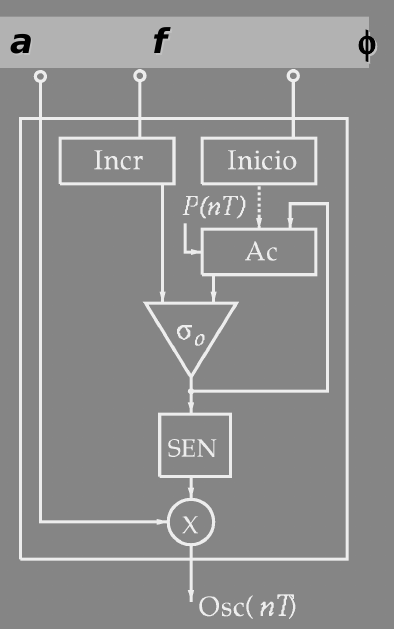
\includegraphics[scale=0.3]{./images/oscilador.png}
  \caption{Esquemático do oscilador padrão}
   \end{figure}
\end{frame}

\begin{frame}
 \frametitle{OsciladorRissetContinuo 3/4}
 \begin{figure}
  \includegraphics[scale=0.4]{./images/osciRisset_esquema.png}
  \caption{Esquemático do osciladot Risset}
   \end{figure}
\end{frame}

\begin{frame}
 \frametitle{OsciladorRissetContinuo 4/4}
 \begin{figure}
  \includegraphics[scale=0.6]{./images/osciRisset_code.png}
  \caption{Construção de OsciladorRissetContinuo}
   \end{figure}
\end{frame}

\begin{frame}
 \frametitle{OsciladorRissetContinuo - gráfico}
 \begin{figure}
  \includegraphics[scale=0.3]{./images/Fi=F0.png}
\caption{Osciladores para Fi = Fc/16}  
    \end{figure}
\end{frame}

\subsubsection{EfeitoRissetContinuo}
\begin{frame}{EfeitoRissetContinuo 1/2}
\begin{itemize}
	\item Conecta vários OsciladoresRissetContinuo definindo as frequências
	como potências de dois de uma frequência base.
	\item possui métodos para configurar todos os parâmetros do efeito
	e um método para obter o som resultante.
	\item na implementação utilizamos 8 harmônicos, começando com Fc/16,
	até Fc e então até 8Fc
\end{itemize}
\end{frame}

\begin{frame}
 \frametitle{EfeitoRissetContinuo 2/2}
 \begin{figure}
  \includegraphics[scale=0.6]{./images/efeitoRisset_code.png}
  \caption{Construção de EfeitoRissetContinuo}
   \end{figure}
\end{frame}


\section{Interface Gráfica}
\begin{frame}
 \frametitle{Interface Gráfica}
 \begin{figure}
  \includegraphics[scale=0.4]{./images/gui.png}
  \caption{Interface Desenvolvida}
   \end{figure}
\end{frame}
\section{Documentação e Referências}
\begin{frame}
  \frametitle{Documentação e Referências}
  \begin{itemize}
  \item \href{../doc/index.html}{Documentação produzida com javadoc}
  \item \href{http://www.cic.unb.br/docentes/lcmm/sintese/javadoc/}{Documentação da API sintese}
  \item \href{http://hebb.mit.edu/courses/9.29/2003/athena/auditory/risset.html}{CIRCULARITY IN PITCH JUDGEMENT, MIT, Introduction to Computational Neuroscience}
  \end{itemize}
\end{frame}





\end{document}
